\section{Attention}

\begin{frame}[c]{Attention in Transformer}
    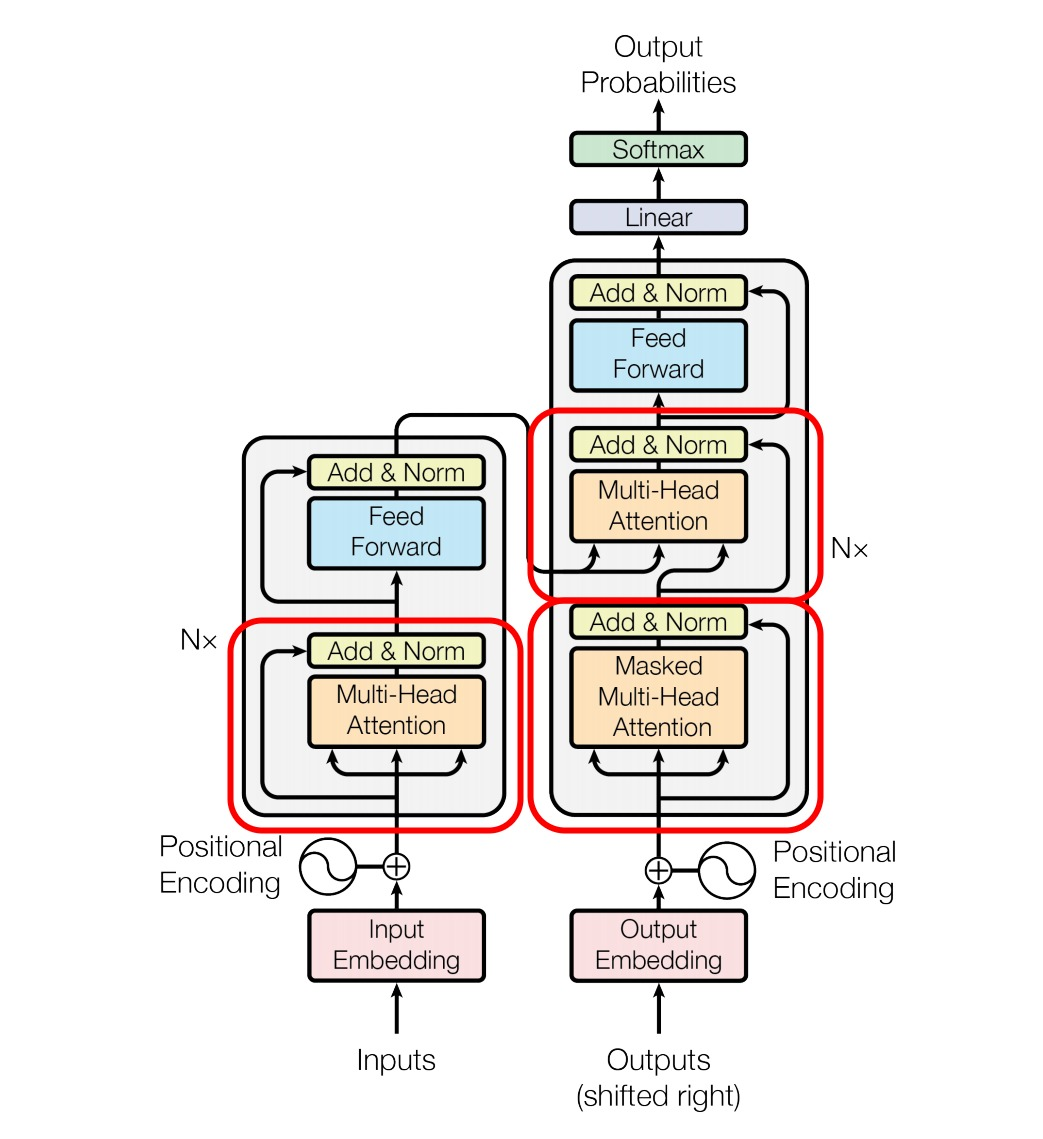
\includegraphics[height=0.9\textheight]{transformer_attention}
\end{frame}


\subsection{Basic Attention}

\begin{frame}[c]{Basic Attention}
    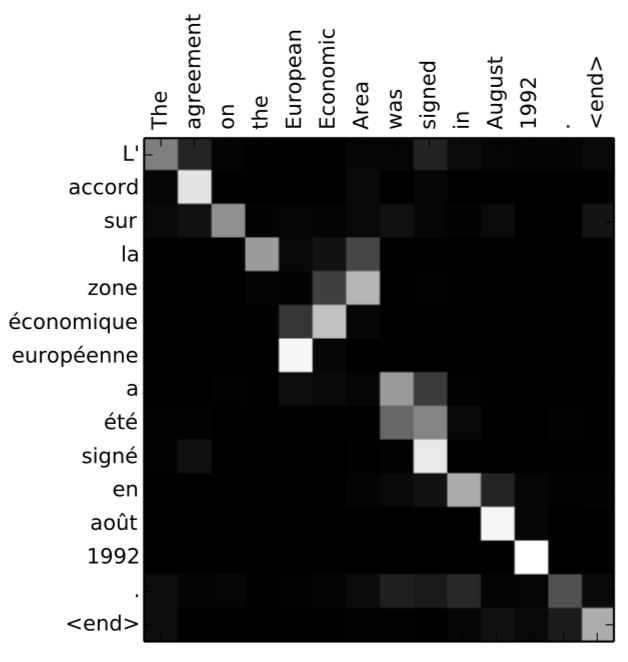
\includegraphics[height=0.85\textheight]{neural-alignment} \\
    Image Source: \cite{bahdanau_neural_2016}
    \pnote{
        Attention existed before the transformer \\
        architecture, but was used in combination \\
        with recurrent neural networks. \\ \\
        As seen here, it focuses on what is learned relevant
    }
\end{frame}

\begin{frame}[c]{Attention Mechanism}
    \large
    $$attention(Q, K, V) = softmax(\frac{QK^T}{\sqrt{d_k}})V$$
    \pause
    where
    $$Q = W_Q\textcolor{blue}{x}, K = W_K\textcolor{blue}{x}, V = W_V\textcolor{blue}{x}, \text{ and } d_k \text{ query-size}$$
    for self-attention \pause and
    $$Q = W_Q\textcolor{blue}{x}, K = W_K\textcolor{red}{y}, V = W_V\textcolor{red}{y}$$
    for encoder-decoder cross-attention
    \pnote{
        d_k is query-size dimension
    }
\end{frame}


\begin{frame}[c]{Scaled Dot-Product Attention}
    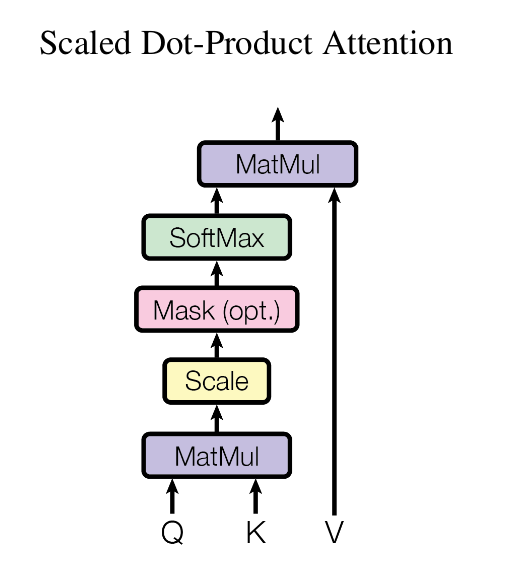
\includegraphics[height=0.9\textheight]{scaled_dot_attention}
    Image Source: \cite{vaswani_attention_2017}
\end{frame}


\subsection{Multi-Head Attention}
\begin{frame}[c]{Multi-Head Attention}
    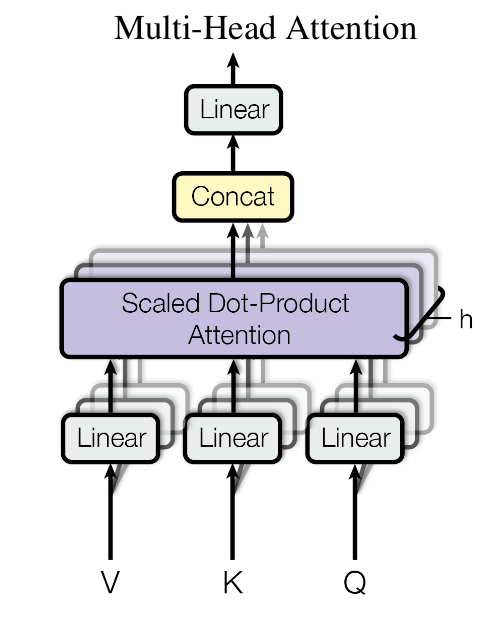
\includegraphics[height=0.9\textheight]{multi_head_attention}
    Image Source: \cite{vaswani_attention_2017}
    \pnote{
        As I understand it, MHA is for splitting the
        embedding space in different partitions, ensuring that each part get's
        at least a certain amount of 'activation'. This can increase
        performance considerably, but effectively it doesn't do
        anything different. Effectively black magic, but seems to
        work.
    }
\end{frame}

\subsection{Masked Attention}
\begin{frame}[c]{Masked Attention}
    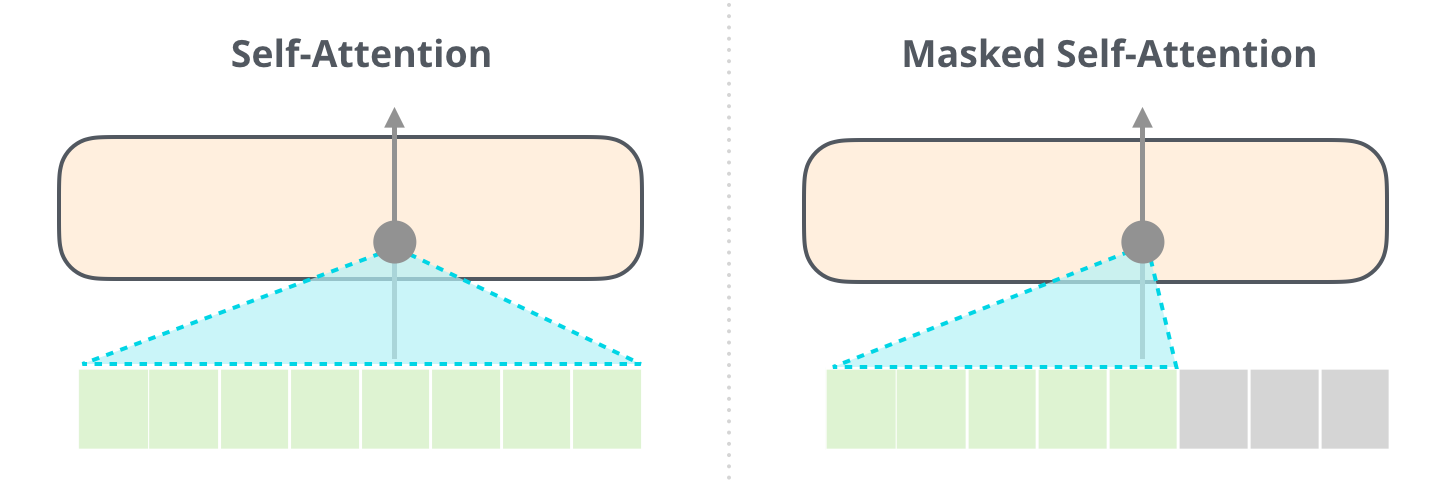
\includegraphics[width=\textwidth]{masked-self-attention} \\
    Image Source: \cite{alammar_illustrated_2019}
\end{frame}

